\section{Аналитические раздел}

\subsection{Равномерное распределение}

\textbf{Равномерное распределение} --- 
распределение случайной величины, принимающей значения, принадлежащие некоторому промежутку конечной длины, 
характеризующееся тем, что плотность вероятности на этом промежутке всюду постоянна.\\

Функция распределения:

\begin{equation*}
	F_X (x) =
	\begin{cases}
		0,& x < a \\
		\frac{x - a}{b - a},& a \le x < b \\
		1,& x \geq b \\
	\end{cases}
\end{equation*}


Плотность распределения:

\begin{equation*}
	f_X (x) =
	\begin{cases}
		\frac{1}{b-a},& x \in [a,b] \\
		0,& x \notin [a, b] \\
	\end{cases}
\end{equation*}

Равномерное распределение обозначается $X \sim R[a, b]$.

\subsection{Распределение Пуассона}

\textbf{Распределение Пуассона} --- 
распределение дискретного типа случайной величины, представляющей собой число событий, 
произошедших за фиксированное время, при условии, 
что данные события происходят с некоторой фиксированной средней интенсивностью и независимо друг от друга.

Функция распределения:

\begin{equation*}
    \lambda^x \frac{\exp(-\lambda)}{x !}
\end{equation*}

Функция плотности:

\begin{equation*}
    \sum_{i=0}^{x} \frac{\lambda^i \exp(-\lambda)}{i!}
\end{equation*}

\section{Результаты работы}

\subsection{Равномерное распределение}

\begin{figure}[h!]
	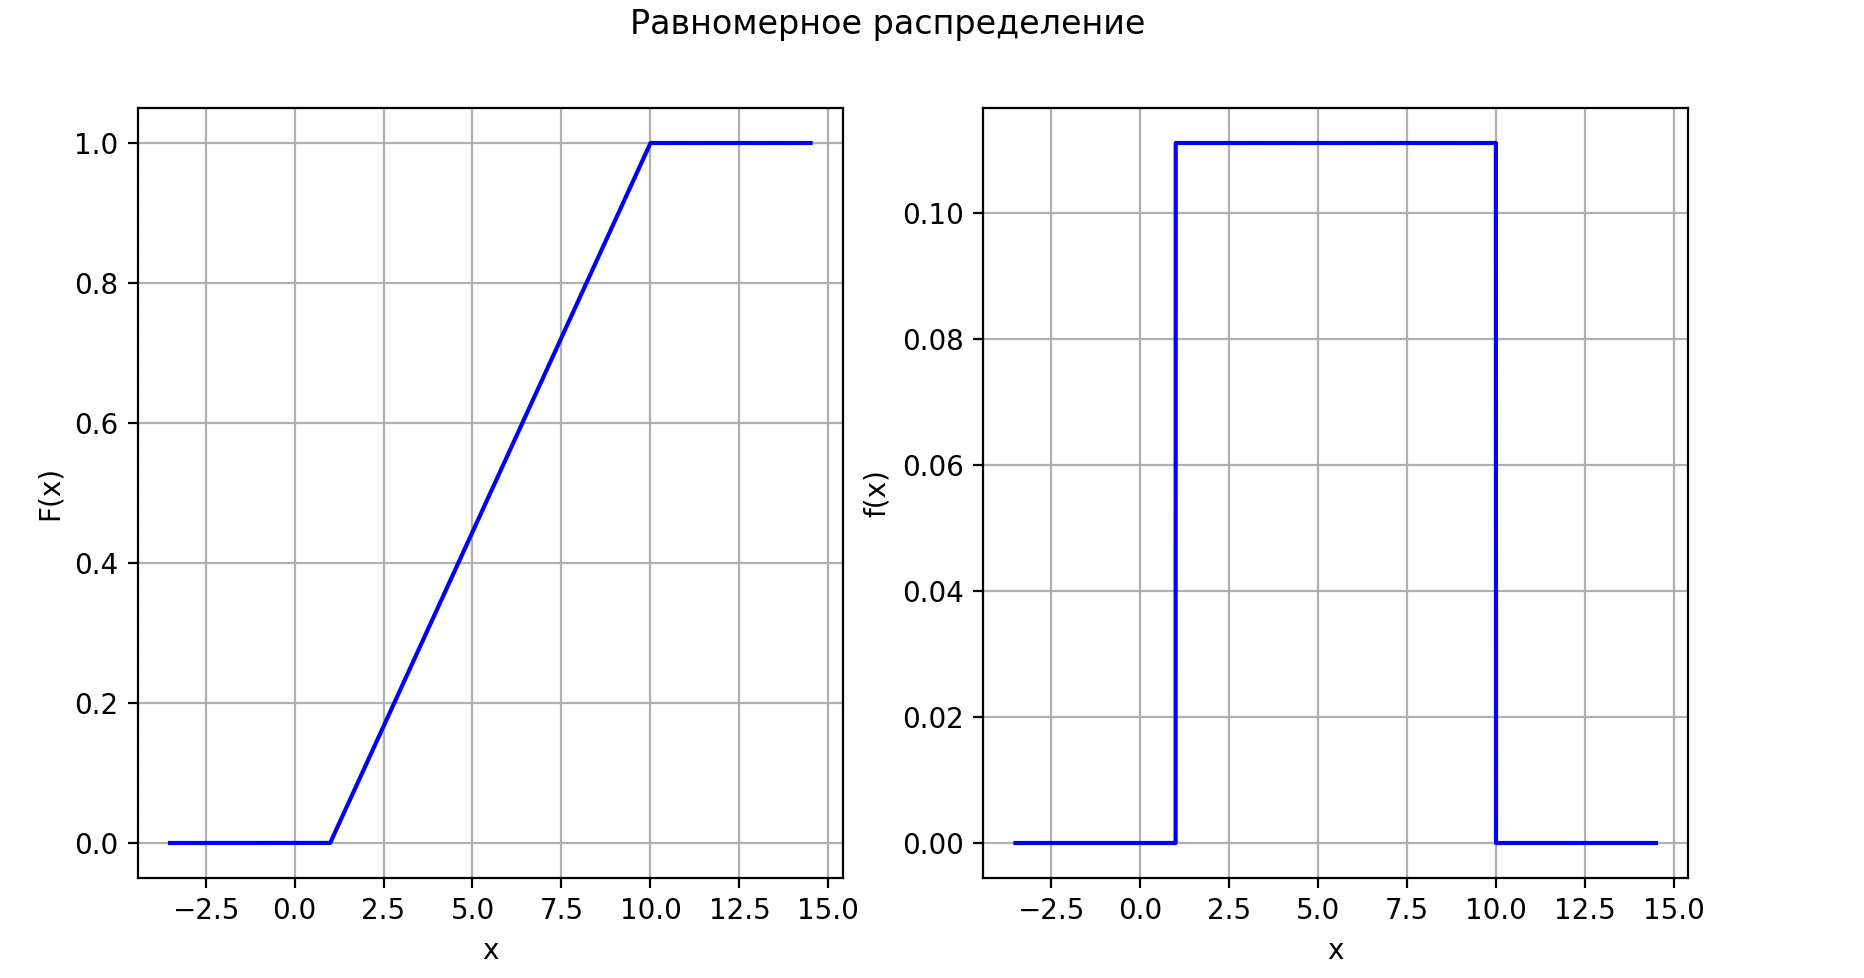
\includegraphics[width=\linewidth]{assets/images/ravn.png}
	\caption{Равномерное распределение при $a=1$, $b=10$}
	\label{fig:r1}
\end{figure}

\subsection{Распределение Пуассона}

\begin{figure}[h!]
	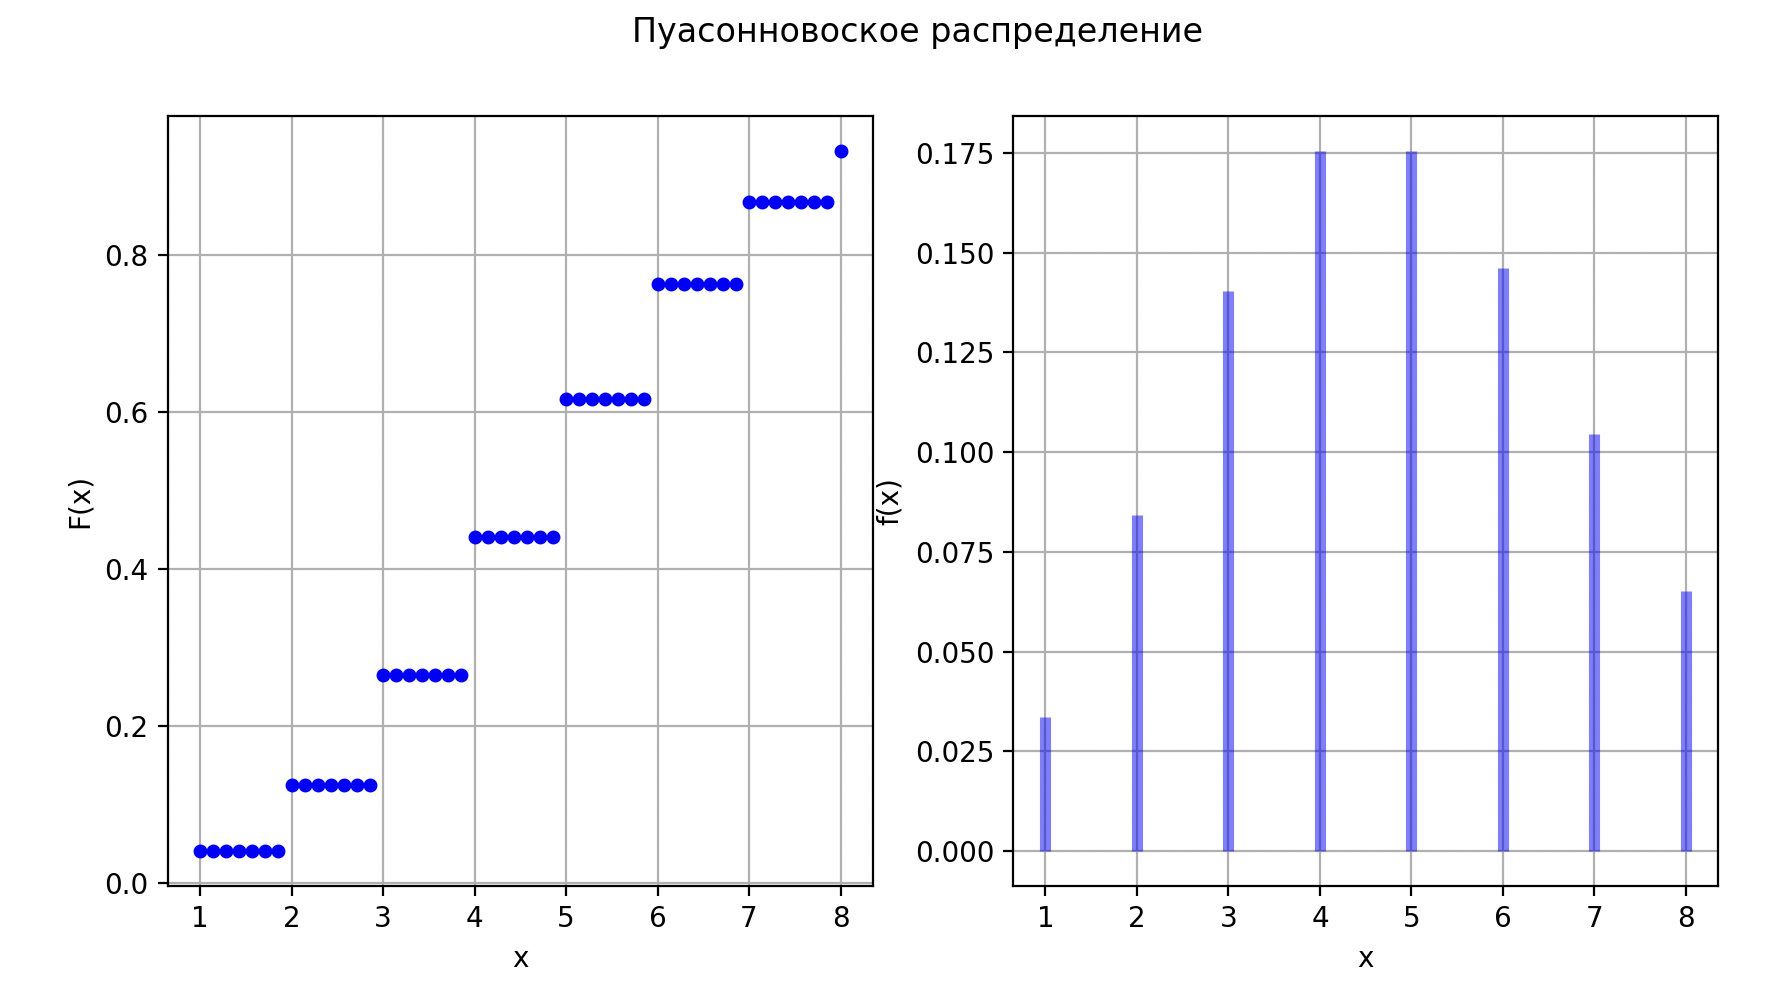
\includegraphics[width=\linewidth]{assets/images/poisson.png}
	\caption{Распределение Пуассона при $\mu=5$}
	\label{fig:r2}
\end{figure}